\documentclass[aspectratio=169, 12pt]{beamer}

\usepackage[utf8]{inputenc}
\usepackage[T1]{fontenc}
\usepackage[catalan]{babel}
\usepackage{lmodern}
\usepackage{amsmath,amssymb}
\usepackage{graphicx}
\usepackage{bm}

\uselanguage{Catalan}
\languagepath{Catalan}
\usecolortheme{seahorse}
\setbeamertemplate{navigation symbols}{}

\let\P\relax
\DeclareMathOperator{\P}{P}
\DeclareMathSymbol{,}{\mathpunct}{operators}{"2C}
\renewcommand{\vec}[1]{\mathbf{\bm #1}}
\DeclareMathOperator{\gr}{gr}
\newcommand{\R}{\mathbb{R}}
\newcommand{\abs}[1]{\left\lvert #1 \right\rvert}

\title{Passejos aleatoris en grafs}
\author{Gerard Castro, Kim López, Ga\l.la Mora, Arnau Mas}
\date{5 de desembre de 2018}

\begin{document}
\begin{frame}
	\titlepage
\end{frame}

\begin{frame}
	\frametitle{Esquema}
	\tableofcontents

\end{frame}

\section{Introducció}

\begin{frame}
	\frametitle{Definició}
	\begin{block}{Definició}
		Un \emph{passeig aleatori} a un graf \( G \) és una seqüència de vèrtexs \( v_1, v_2, \cdots, v_n, \cdots \), tal que \( v_kv_{k+1} \) es tria uniformement d'entre les arestes incidents a \( v_k \).
	\end{block}
\end{frame}

\begin{frame}
	\frametitle{Aspectes probabilístics}
	\( V(t) \) és la variable aleatòria que representa la posició del passeig a l'instant \( t \) \pause

	Les probabilitats de transició \[ \P(V(t) = u \mid V(t - 1) = v) \] determinen el passeig: \pause
	\begin{equation*}
		\P(V(t) = u) = \sum_{v \in V(G)} \P(V(t) = u \mid V(t - 1) = v) \, \P(V(t - 1) = v).
	\end{equation*}
\end{frame}

\begin{frame}
	\frametitle{Probabilitats de transició}
	Com que \[ \P(V(t) = u \mid V(t - 1) = v) = \frac{a(u,v)}{\gr(v)}, \] \pause
	tenim
	\[ P(V(t) = u) = \sum_{v \in V(G)} \frac{a(u,v)}{\gr(v)}P(V(t - 1) = v). \]
\end{frame}

\begin{frame}
	\frametitle{Un exemple}
	\begin{columns}
		\begin{column}{0.5\textwidth}
			\only<2>{
				\[ \P(V(0) = i_1) = 1 \]
			}
			\only<3>{
				\begin{align*}
					\P(V(1) = i_2) & = \P(V(1) = i_3) \\
												 & = \P(V(1) = i_4) = \frac{1}{3}
				\end{align*}
			}
			\only<4>{
				\[ \P(V(3) = i_1) = 1 \]
			}
		\end{column}

		\begin{column}{0.5\textwidth}
			\centering
			\only<2,4>{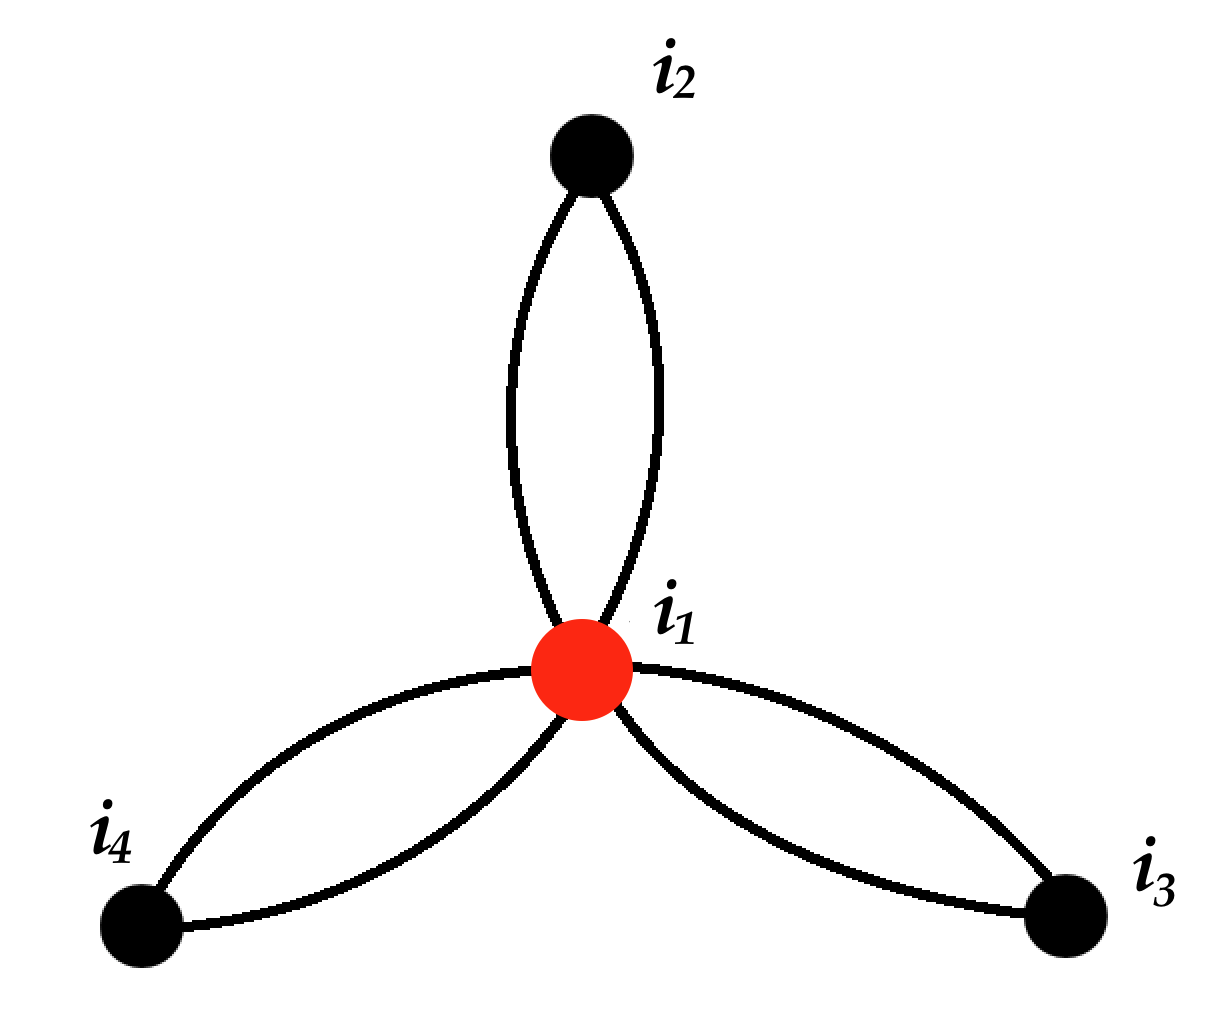
\includegraphics[scale = 0.15]{exemple-1.png}}
			\only<3>{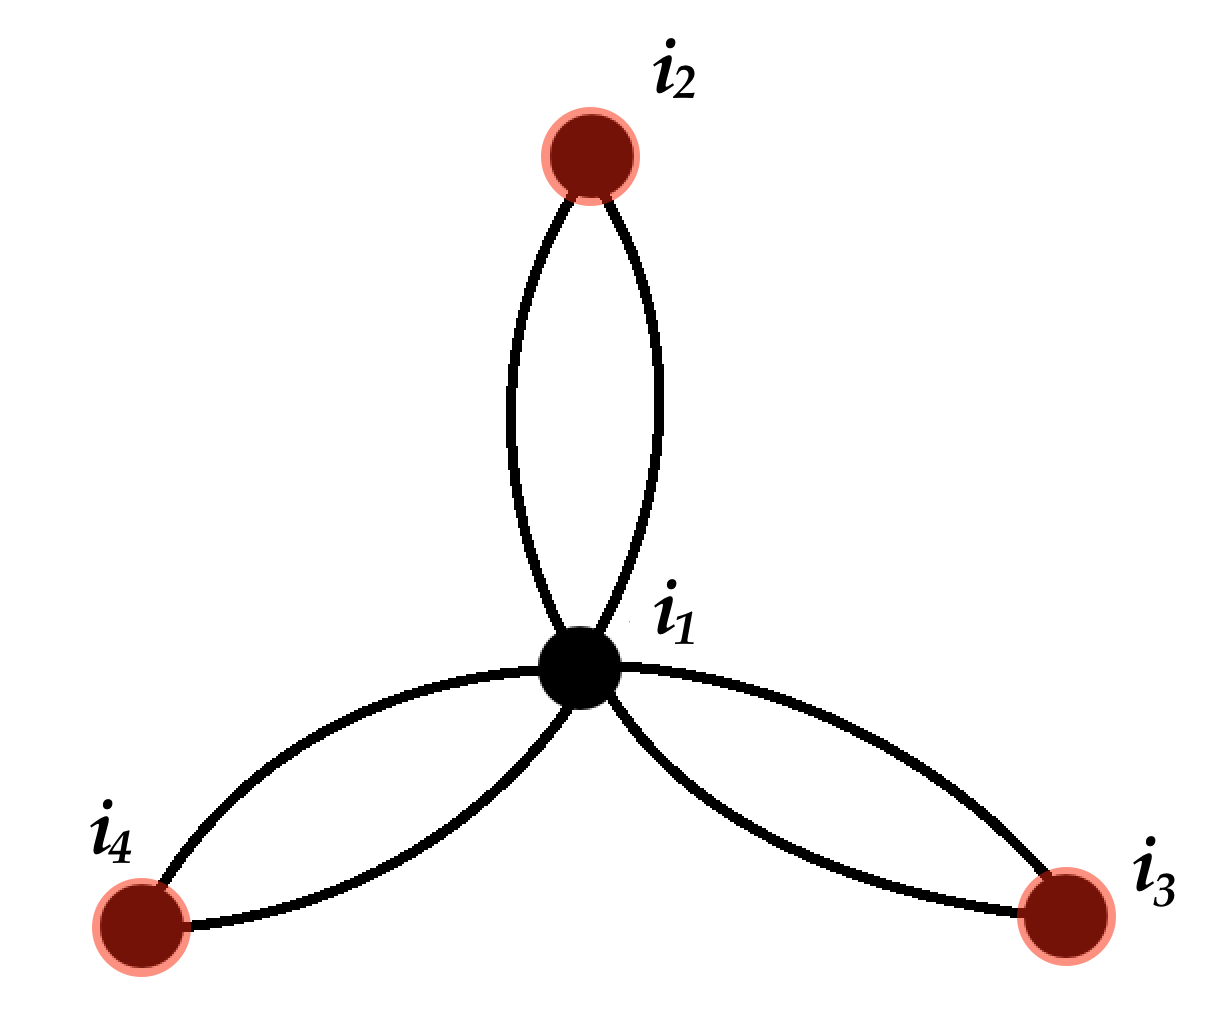
\includegraphics[scale = 0.15]{exemple-2.png}}

		\end{column}
	\end{columns}

\end{frame}

\begin{frame}
	\frametitle{Matriu de transició}
	Definim \( \vec{p}_t \in \R^{V(G)} \) com \( \vec{p}_t(u) = P(V(t) = u) \). \pause Aleshores, en forma matricial \[ \vec{p}_t = AD^{-1} \vec{p}_{t - 1}. \] \( A \) és la matriu d'adjacència i \( D \) la matriu dels graus. \( P = AD^{-1} \) és la \emph{matriu de transició}. \pause

	Per tant \[ \vec{p}_t = P^t \vec{p}_0. \]
\end{frame}

\begin{frame}
	\frametitle{Un exemple}
	\begin{columns}
		\begin{column}{0.5\textwidth}
			\only<2>{
				\begin{equation*}
					A = \begin{pmatrix}
						0 & 1 & 1 & 1 \\
						1 & 0 & 0 & 0 \\
						1 & 0 & 0 & 0 \\
						1 & 0 & 0 & 0
					\end{pmatrix} 
					\, D = \begin{pmatrix}
						6 & 0 & 0 & 0 \\
						0 & 2 & 0 & 0 \\
						0 & 0 & 2 & 0 \\
						0 & 0 & 0 & 2
					\end{pmatrix}
				\end{equation*}
				\begin{equation*}
					P = \begin{pmatrix}
						0 & 1 & 1 & 1 \\
						1/3 & 0 & 0 & 0 \\
						1/3 & 0 & 0 & 0 \\
						1/3 & 0 & 0 & 0
					\end{pmatrix}
				\end{equation*}
			}
			\only<3>{
				\begin{equation*}
					\vec{p}_0 = (1,0,0,0)	
				\end{equation*}
			}
			\only<4>{
				\begin{equation*}
					\vec{p}_1 = \left(0,\frac{1}{3},\frac{1}{3},\frac{1}{3}\right) = P\vec{p}_0	
				\end{equation*}
			}
			\only<5>{
				\begin{equation*}
					\vec{p}_2 = (1,0,0,0)	= P\vec{p}_1 = P^2\vec{p}_0
				\end{equation*}
			}
		\end{column}

		\begin{column}{0.5\textwidth}
			\centering
			\only<2,3,5>{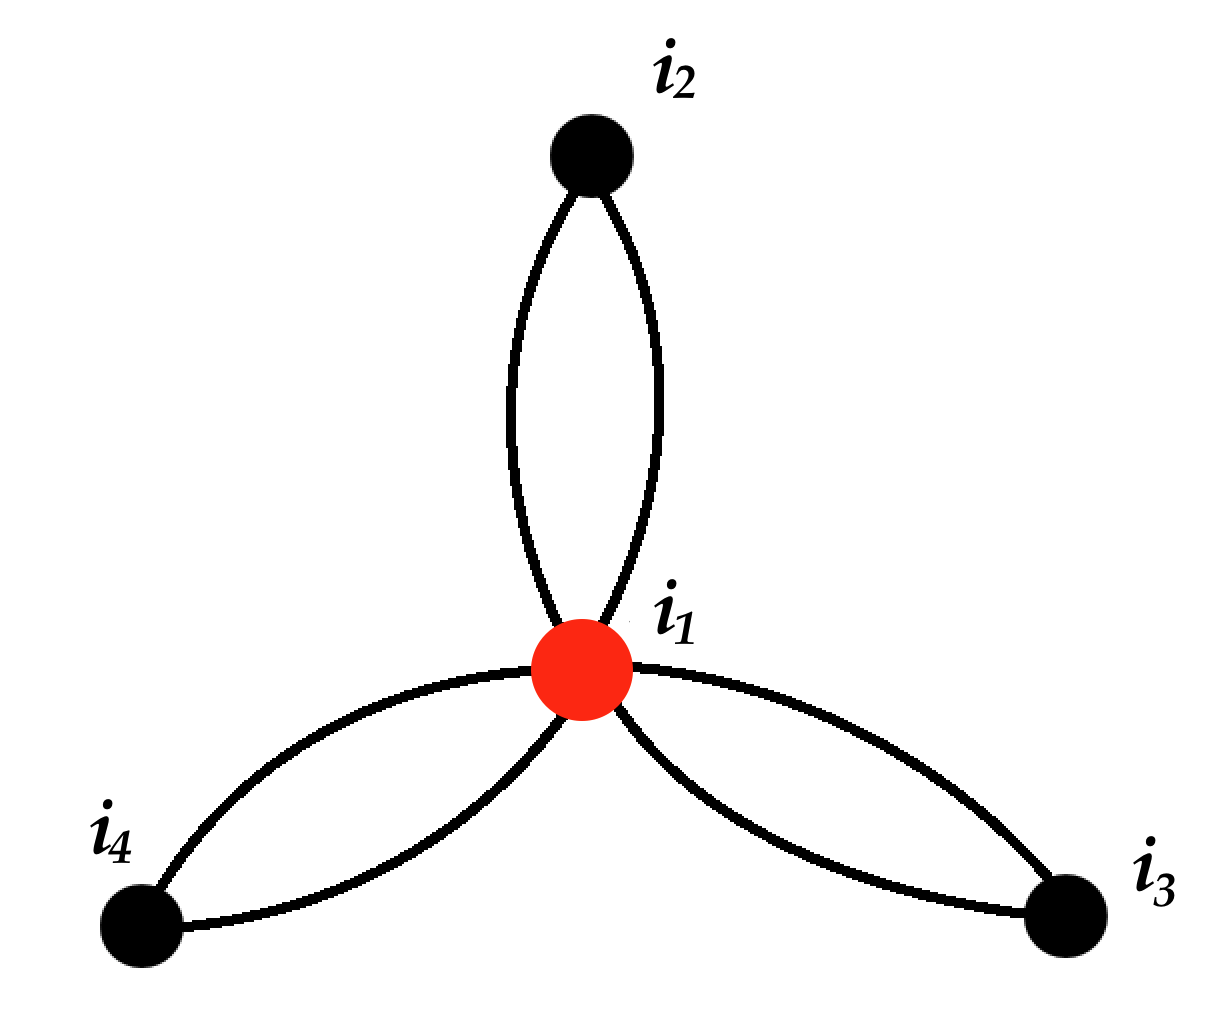
\includegraphics[scale = 0.15]{exemple-1.png}}
			\only<4>{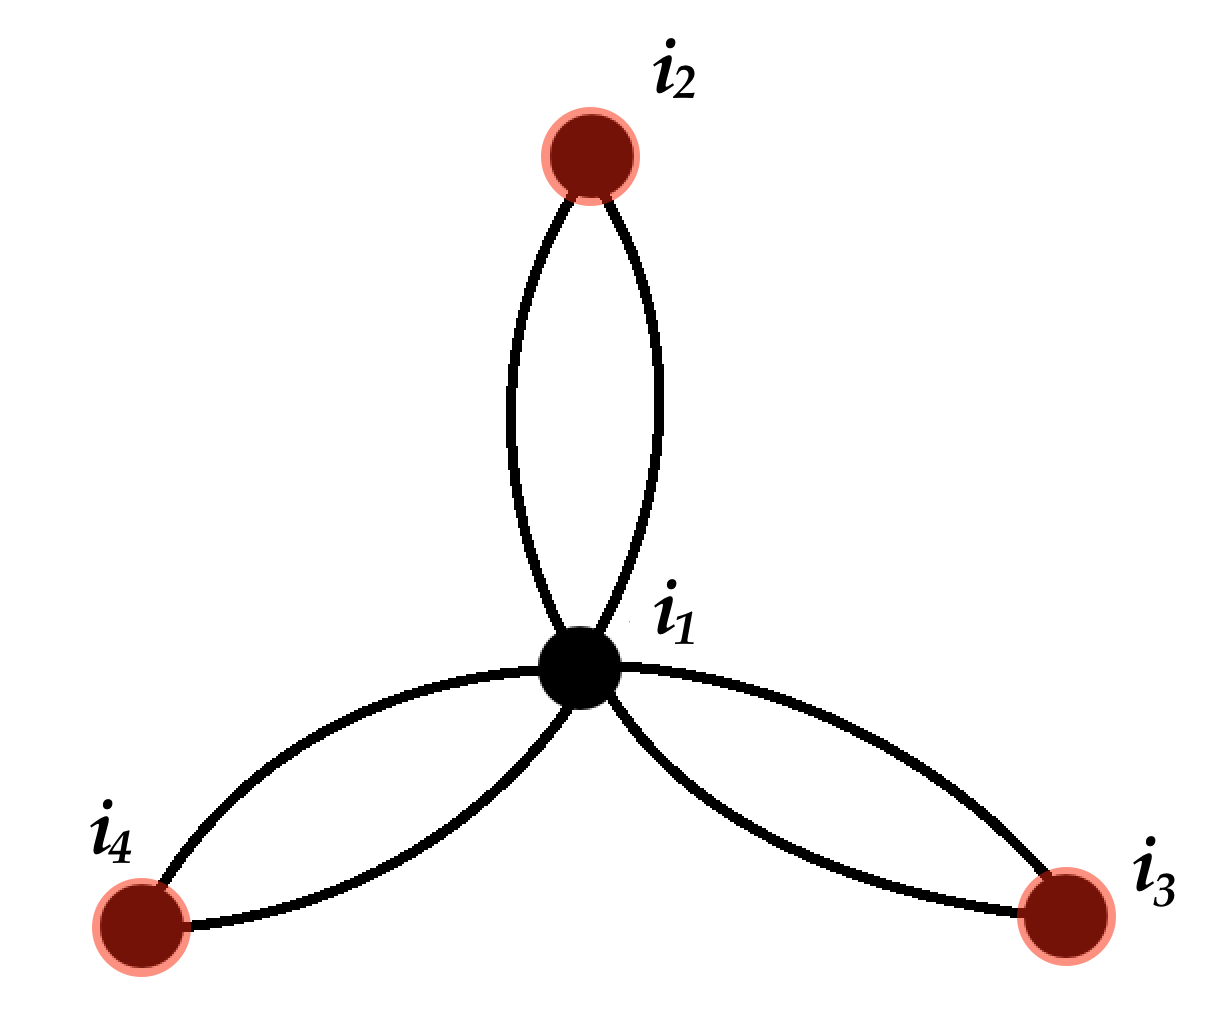
\includegraphics[scale = 0.15]{exemple-2.png}}

		\end{column}
	\end{columns}

\end{frame}

\section{Resultats principals}

\begin{frame}
	\frametitle{Distribució estacionària}
	Com és el passeig per a temps grans? \pause

	\begin{block}{Definició}
		Una distribució és \emph{estacionària} si \( \P(V(t) = u) = \P(V(t - 1) = u) \) per tot \( u \in V(G) \).
	\end{block} \pause

	En termes de la matriu de transició, \[ P\vec{\pi} = \vec{\pi}. \]
\end{frame}

\begin{frame}
	\frametitle{Existència i unicitat de distribucions estacionàries}
	\begin{theorem}
		Tot graf connex admet una única distribució estacionària.
	\end{theorem}
	\pause

	\begin{proof}
		\( \vec{\pi} \) estacionària. Veurem que \( \vec{\pi}(u) \propto \gr{u} \). \pause Sigui \( u^\ast \) tal que \( \frac{\vec{\pi}(u^\ast)}{\gr(u^\ast)} \) és màxim: \pause 
		\begin{equation*}
			\vec{\pi}(u^\ast) = \sum_{v \in V(G)} \frac{a(u^\ast,v)}{\gr(v)} \vec{\pi}(v) \pause \leq \frac{\vec{\pi}(u^\ast)}{\gr(u^\ast)} \sum_{v \in V(G)} a(u^{\ast},v) \pause = \vec{\pi}(u^\ast)
		\end{equation*}
		Per tant \( \frac{\vec{\pi}(v)}{\gr(v)} = \frac{\vec{\pi}(u^\ast)}{\gr(u^\ast)} \) per tot \( v \) adjacent a \( u^\ast \). 
	\end{proof}
\end{frame}

\begin{frame}
	\frametitle{Existència i unicitat de distribucions estacionàries}
	\begin{proof}
		Per \( v \) no adjacents, com que \( G \) és connex, per \( n \) prou gran, \[ \P(V(t + n) = u^\ast \mid V(t) = v) > 0 \] per tot \( v \in V(G) \), i podem reproduir l'argument ja que \( \vec{\pi} = P^n \vec{\pi} \) per tot \( n \). \pause

		Com que \( \vec{\pi}(u) \propto \gr(u) \), normalitzant
		\begin{equation*}
			\vec{\pi}(u) = \frac{\gr(u)}{\sum_{v \in V(G)} \gr(v)} \pause = \frac{\gr(u)}{2 \abs{E(G)}}
		\end{equation*}

	\end{proof}
\end{frame}
\section{PageRank}

\section{Altres aplicacions}

\section{Problemes oberts}
\end{document}
